\documentclass[12pt]{article}
\usepackage{jcappub}
\usepackage{amsmath}
\usepackage{graphicx}
\usepackage{mathtools} %For summations with limits
\usepackage{multicol} %For multiple columns
\setlength{\columnsep}{1cm}


\title{The Distribution of Vacua in Random Landscape Potentials}

\author{Low Lerh Feng,}
\author{Shaun Hotchkiss}
\author{and Richard Easther}

\emailAdd{lerh.low@auckland.ac.nz}
\emailAdd{s.hotchkiss@auckland.ac.nz}
\emailAdd{r.easther@auckland.ac.nz}

\newcommand{\re}[1]{\textcolor{blue}{[{\bf RE}: #1]}}
\newcommand{\lfl}[1]{\textcolor{red}{[{\bf LL}: #1]}}


\affiliation{Department of Physics,\\ University of Auckland, \\Private Bag 92019,\\ Auckland, New Zealand}



\abstract{ Landscape cosmology posits the existence of a convoluted, multidimensional, scalar potential -- the eponymous ``landscape'' -- with vast numbers of metastable minima. The huge number of minima supported by landscape potentials motivate arguments that landscape cosmology reduces tuning problems associated with a small but non-zero vacuum energy by providing a framework in which anthropic or ``environmental'' selection is plausible. Random matrices and random functions in many dimensions can be used to discuss  conceptual issues associated with landscape scenarios; here we explore the distribution of minima as a function of vacuum energy in an $N$-dimensional Gaussian random potential. We derive a ``likelihood''  for the density of minima in $N$ dimensions, showing that after rescalings its properties are fully defined by $N$ and a  single free parameter, $\sigma_2$. We use this likelihood to compute the likelihood of finding minima as a function of the amplitude of the landscape, and to compute $P(\Lambda)$, the distribution function of vacuum energies in these scenarios. \lfl{Aren't $P(\Lambda)$ and the likelihood of finding minima as a function of the amplitude synonymous?}}

\begin{document}



\maketitle

\section{Introduction}

Over the last two decades cosmology has developed in apparently paradoxical directions. Observationally, the rise of ``precision cosmology'' makes it possible to measure key parameters to within a few percent, setting stringent tests for the detailed evolutionary narrative given by concordance $\Lambda$CDM cosmology\cite{Planck2018,DES}. Conversely, theoretical investigations of both slow-roll inflation and string theory along with a non-zero dark energy density motivates  theoretical investigations of multiverse-like scenarios. In particular, studies of stochastic inflation \cite{Linde1986,Adshead2007} suggest that the mechanism that produces astrophysical density perturbations could also support {\em eternal inflation\/}, generating infinite numbers of  {\em pocket universes\/} \cite{Guth2001}. Likewise, studies of flux compactified string vacua points to a possible  {\em landscape\/} \cite{Susskind2003} or {\em discretuum\/} \cite{Bousso2000}   of vacua within the theory. These developments open the door to anthropic explanations of the non-zero vacuum energy density, insofar as a value that was  exactly zero could be more plausibly explained by an unknown symmetry. 

Stochastic (or eternal) inflation implies the existence of a multiverse composed of many pocket universes, but this does not require that the ``low energy" (i.e. LHC scale) physics or vacuum energy differs between pockets:  the naive quadratic inflation model is potentially eternal, but has a unique vacuum.  By contrast, landscape models have multiple vacua which can, in principle, be populated by stochastic inflation or tunneling. The string landscape, built on the plethora of flux-stablilsed vacua that exist inside Calabi-Yau spaces, is well-known but  is not necessarily a unique realisation of this scenario. The complexity of the landscape  and the vast number of vacua it supports is the basis of its purported explanatory power: the number of vacua is almost uncountably large (e.g. $10^{500}$ or greater \cite{Douglas2003}) and any value of the vacuum energy can thus conceivably be realised within it. 
 
The detailed properties of any possible landscape are almost entirely unknown -- it is still unclear whether any specific stringy construction  realises  the $SU(3) \times SU(2) \times U(1)$ gauge group of the Standard Model.  More recently the Swampland Conjecture suggests that all stable minima of the theory might actually be ``underwater'' \cite{Agrawal2018},  located at negative values of $\Lambda$. If true, this would require that the cosmological dark energy was underpinned by dynamical quintessence-like evolution.  

An alternative approach to   landscape scenarios is to strip them down to their barest essence -- by realising multiverse cosmology within a {\em random\/} multidimensional ($N\sim100$ or more) potential of interacting scalar fields.\footnote{Random is used here in the  context of random function theory \cite{GRF1, GRF2, GRF3}.  We refer to random functions rather than random fields, the nomenclature often seen in the mathematical literature, to avoid confusion with the individual scalar fields that are coupled by the potential.}  In this approach the ``large $N$'' properties of the multidimensional landscape actually provides leverage that can be used to develop an understanding of its properties. The first steps in this direction were taken by Aazami and Easther \cite{Aazami2006}, investigating ensembles of Hessian matrices describing extrema in a random landscape.  At  a minimum in the landscape the eigenvalues of the Hessian are all positive. For simple random matrix distributions eigenvalues are likely to be evenly distributed between positive and negative values with fluctuations away from this situation being strongly suppressed at even moderate values of $N$, suggesting that the number of minima is super-exponentially smaller than the number of saddles. This simple argument is actually incorrect; the individual entries of the Hessians matrices of random functions are correlated and therefore not drawn from identical, independent distributions, violating a common premise of random matrix theory \cite{Battefeld2012,Easther2016}. That said, this  overall approach has been widely pursued and has now been extended in a number of directions \cite{Easther2006, Frazer2011, Henry2009, Marsh2013, Agarwal2011,Yang2012,Masoumi2016,Yamada2018}. This line of enquiry has also motivated studies of the properties of random matrices and random functions at large $N$.\cite{Bray2007,Dean2008,Majumdar2009,Bachlechner2014,Battefeld2012,Fyodorov2013,Masoumi2017} Similar mathematical problems arise in statistical mechanics, string theory, and complex dynamics.\cite{Fyodorov2004,Douglas2004,Douglas2006,Fyodorov2007,Fyodorov2012,Fyodorov2018,Ros2019}

%The theory of inflation is the current best explanation for certain perplexing observations of the Universe, such as the monopole problem, horizon problem, and flatness problem. Inflation is thought to be caused by a scalar field, but the exact nature of this field is shrouded in unknowns. The simplest possibility is a one-dimensional scalar field analogous to the gravitational potential; however multidimensional scalar fields are also possible. In particular, string theory predicts the existence of a highly complex, $O(100)$ dimensional scalar field known as the \emph{landscape}. The string landscape is so complex that quantitative predictions are hard to extract; as a result, most studies of the landscape assume it is a Gaussian random field

In conventional inflationary scenarios, accelerated expansion occurs when the gradient of the potential is small (so-called ``slow-roll"), and trajectories typically end in a minimum of the potential. If this is the global minimum, the end-state is stable. However,  bubbles of space can tunnel from  a local minimum to lower-lying vacua, rendering local minima metastable, although often with lifetimes much greater than the age of the universe. If this local minimum has a positive vacuum energy it will contribute an apparent cosmological constant term to observers within the universe. Accordingly, we are interested in the probability of finding a minimum at potential values $F >0$. In particular, we show that for some region of parameter space, a random potential with $10^M$ minima (where $M$ is a number of order $\mathcal{O}(100)$) can also have $P(F > 0|min) < 10^{-M}$, so that it is conceivable that these scenarios have no metastable solutions with  positive vacuum energy. Further, these considerations may be used to establish a weakly non-uniform measure on the vacuum energy. Finally, the methods we use also provide a likelihood for the eigenvalues at minima, allowing us to infer their shapes.

We proceed from a generalisation of the Kac-Rice formalism \cite{Kac1943,Rice1945} and the  machinery developed by Bond, Bardeen, Kaiser and Szalay  \cite{BBKS}  for studying the statistics of Gaussian random fields in  cosmological perturbation theory   to $N$ dimensions.  We then build a ``ladder'' of numerical techniques, proceeding from exactly evaluated integrals at small $N$ to Monte Carlo evaluation, and then to numerical evaluations of Gaussian approximations to the underlying integrals out to $N=100$. These techniques can be generalised to other, more complex questions about trajectories in these potentials, and give information about the ``shapes'' of minima which may inform analyses of tunnelling. We show that $P(\Lambda)$, the probability density function for the vacuum energy, depends on the dimensionality $N$ and a single free parameter for a Gaussian random landscape, and this parameter can be computed directly from the power spectrum. Finally, we discuss the implications of these results for landscape cosmology and notions of anthropic selection. 

\section{Random Potentials in $N$ Dimensions}

We begin by developing an $N$-dimensional analogue of the treatment of three dimensional random functions due to Bardeen, Bond, Kaiser and Szalay (henceforth BBKS) \cite{BBKS}, generalising their derivation and keeping their notation as far as possible.   An $N$-dimensional scalar-valued function $F(r)$ is a set of values that fill each point of $N$-dimensional space. The function is \emph{random} if its values depend on a probability distribution function,
%
\begin{equation}
P[F(r_1), F(r_2), \ldots, F(r_m)]dF(r_1)dF(r_2)\ldots dF(r_m)
\end{equation}
%
\noindent where $r_i$ is a position in $N$ dimensional space. This corresponds to the probability that the function takes value $F(r_1) \pm dF(r_1)$ at position $r_1$, $F(r_2) \pm dF(r_2)$ at position $r_2$, and so on. 
%
The function is \emph{Gaussian random} if the probability distribution function is an $N$-dimensional Gaussian function,
%
\begin{equation} \label{MultivariateGaussian}
\begin{split}
P(y_1,\ldots,y_N)dy_1\ldots dy_N &= \frac{e^{-Q}}{[(2\pi)^N \mathrm{det}(M)]^{1/2}} dy_1\ldots dy_N \, ,\\
Q &\equiv \frac{1}{2} \sum \Delta y_i (M^{-1})_{ij} \Delta y_{ij} \, .\\
\end{split}
\end{equation}
%
Here $M$ is the \emph{covariance matrix}, 

\begin{equation}
M_{ij} \equiv \langle \Delta y_i \Delta y_j \rangle
\end{equation}

\noindent while $\Delta y_i$ is the difference between the measured value and the average, $\Delta y_i \equiv y_i - \langle y_i \rangle$. For a Gaussian random function, the probability distribution only depends on $M$, which in turn only depends on the two-point correlation function $\langle \Delta y_i \Delta y_j \rangle$. In other words, the two-point correlation function completely determines the statistical properties of the Gaussian random function.

In our application, the function value we're interested in is the potential of the landscape, so henceforth we will replace $y$ with $F$. The two-point correlation function is, by definition, the Fourier transform of the power spectrum $P(k)$,

\begin{equation}
\langle F(\vec{x}) F(\vec{y}) \rangle = \frac{1}{(2\pi)^N} \int d^Nk e^{i \vec{k} \cdot (\vec{x}-\vec{y})} P(k)
\end{equation}

\noindent where $\vec{x}$ and $\vec{y}$ are directional vectors. We define moments of the power spectrum by

\begin{equation} \label{moments}
\sigma_n^2 = \frac{1}{(2\pi)^N}\int d^Nk (k^{2})^n P(k)
\end{equation}

\noindent i.e. $\langle FF \rangle = \sigma_0^2$. We can differentiate Eq. \ref{moments} and set $\vec{x} = \vec{y}$ to get

\begin{align*}
\langle \eta_{i}(\vec{x})\eta_{j}(\vec{x})\rangle &= \frac{1}{(2\pi)^N} \frac{\partial}{\partial x^i}\frac{\partial}{\partial y^j} \int d^Nk e^{i \vec{k} \cdot (\vec{x}-\vec{y})} P(k)\bigg{|}_{\vec{y}=\vec{x}}\\
&= \frac{1}{(2\pi)^N}\int d^Nk k^i k^j P(k)
\end{align*}

\noindent where $\eta_{i}$ indicates the derivative of $F(\vec{x})$ with respect to $x_i$. Because of isotropy (derivatives must be the same in all directions), the right hand side must be proportional to $\delta_{ij}$. Therefore

\begin{align*}
\langle \eta_{\alpha,i}\eta_{\beta,j}\rangle = K \delta_{\alpha,\beta}\delta_{ij} &\rightarrow \delta_{ij}\langle \eta_{\alpha,i}\eta_{\beta,j}\rangle = NK \delta_{\alpha,\beta}=\sigma_1^2\\
&\rightarrow K = \frac{1}{N}\sigma_1^2
\end{align*}

A similar analysis holds for the second derivatives $\xi_{ij}$, and the resulting relations between the various moments of the power spectrum, the function values, and the derivatives are:

%Our analysis is an N-dimensional generalization of Appendix A in Bardeen, Bond, Kaiser and Szalay (henceforth BBKS) \cite{BBKS}. We adopt the same notation, $\eta_i \equiv \frac{\partial \phi}{\partial x^i}, \xi_{ij} \equiv \frac{\partial^2 \phi}{\partial x^i \partial x^j}$. In this notation, the correlations of a Gaussian random function at a random point in N-dimensions are:

\begin{equation} \label{corr}
\begin{split}
\langle FF \rangle &= \sigma_0^2 \\
\langle\eta_i\eta_j\rangle &= \frac{1}{N}\delta_{ij}\sigma_1^2 \\
\langle\phi\eta_{ij}\rangle &= -\frac{1}{N}\delta_{ij}\sigma_1^2 \\
\langle\xi_{ij}\xi_{kl}\rangle &= \frac{1}{N(N+2)}\sigma_2^2(\delta_{ij}\delta_{kl}+\delta_{il}\delta_{jk}+\delta_{ik}\delta_{jl})
\end{split}
\end{equation}

\noindent For $N=3$ this reduces to BBKS's equation A1. 

We define the following vector:

\begin{equation}
\begin{split}
\alpha = \{F,\eta_1,\eta_2,\ldots,\xi_{11},\xi_{22},\ldots,\xi_{NN},\xi_{N-1,N},\xi_{N-2,N},\ldots,\xi_{1N},\xi_{N-2,N-1},\\
\ldots\xi_{1,N-1},\ldots,\xi_{12}\}
\end{split}
\end{equation}

\noindent With this choice for $\alpha$ (equivalent to $\Delta y$ in Eq. \ref{MultivariateGaussian}), the covariance matrix $M_{ij}\equiv\langle\alpha_i\alpha_j\rangle$ and its inverse $K \equiv M^{-1}$ takes the following general form:

\begin{align*}
K_{F, F} &= \frac{\sigma_2^2}{\sigma_0^2\sigma_2^2-\sigma_1^4} \\
K_{F, \xi_{ij}} &= \frac{\sigma_1^2}{\sigma_0^2\sigma_2^2-\sigma_1^4} \\
K_{\eta_i,\eta_j} &= \frac{N}{\sigma_1^2}\\
K_{\xi_{ii},\xi_{ii}} &=  \frac{N(N+2)}{\sigma_2^2} \\
K_{\xi_{ij}, \xi_{ij}} &= \frac{N\sigma_0^2\sigma_2^2-(N+2)\sigma_1^4}{2(\sigma_1^4\sigma_2^2-\sigma_0^2\sigma_2^4)}, (i\neq j)\\
K_{\xi_{ii}, \xi_{jj}} &= \frac{(N(N+1)-2)\sigma_1^4 - N(N+1)\sigma_0^2\sigma_2^2}{2(\sigma_1^4\sigma_2^2-\sigma_0^2\sigma_2^4)}, (i \neq j)\\
\end{align*}

\noindent and all other terms are zero. The probability distribution of $\alpha_i$ is, from Eq. \ref{MultivariateGaussian}

\begin{equation} \label{ProbDistrib}
p(\alpha_i)=\frac{1}{(2\pi)^{N/2}\sqrt{\mathrm{det}M}} e^{-\frac{1}{2}\alpha K \alpha}
\end{equation}
%
We can usually ignore the constant prefactor since we will primarily be concerned with ratios of probabilities.  We adopt the basis
%
\begin{align}
\begin{split}
\label{BasisTransform}
\sigma_2x_1 = -\nabla^2F &= -(\xi_{11}+\xi_{22}+\ldots+\xi_{NN})\\
\sigma_2x_2 &= -(\xi_{11}-\xi_{22})\\
\sigma_2x_3 &= -(\xi_{11}+\xi_{22}-2\xi_{33})\\
\sigma_2x_4 &= -(\xi_{11}+\xi_{22}+\xi_{33}-3\xi_{44})\\
\ldots
\end{split}
\end{align}
%
$x_1, x_2, x_3, \ldots$ are analogous to BBKS's $x, y, z$. Following BBKS, we introduce $\nu = F/\sigma_0$. With this choice of basis, the nonzero correlations are (from Eq. \ref{corr}):
%
\begin{gather}
\langle\nu^2\rangle = 1, \langle x_1^2\rangle=1, \langle x_2^2 \rangle = \langle \xi_{11}^2 -2\xi_{11}\xi_{22} + \xi_{11}^2\rangle = \frac{4}{N(N+2)} \\
\langle x_3^2 \rangle = \frac{12}{N(N+2)}, \ldots, \langle x_n^2 \rangle = \frac{2n(n-1)}{N(N+2)}.
\end{gather}

The factor $\alpha K \alpha$ (equivalent to $Q$ in BBKS) in Eq. \ref{ProbDistrib} takes the form

\begin{equation} \label{Q}
\begin{split}
2Q = \nu^2 + \frac{(x_1-x_*)^2}{1-\gamma^2} + \frac{N(N+2)}{4}x_2^2 + \frac{N(N+2)}{12}x_3^2 + \ldots + \frac{N(N+2)}{2n(n-1)}x_n^2 \\ + \frac{N \pmb{\eta}\cdot \pmb{\eta}}{\sigma_1^2} + \sum_{i,j;i > j}^N\frac{N(N+2)\xi_{ij}}{\sigma_2^2}
\end{split}
\end{equation}

\noindent where $x_* \equiv \gamma \nu$ and $\gamma = \frac{\sigma_1^2}{\sigma_2 \sigma_0}$. This is the equivalent of BBKS Eq. (A4) for $N$-dimensions. Note the first two terms remain constant for all $N$, but the remaining terms vary. The $\eta$ terms are zero at minima by definition, while the off-diagonal $\xi_{ij}$ terms can be Euler-rotated away by choosing an appropriate set of axes. The $\xi$ matrix is already symmetric (by rotational symmetry), and Euler rotation turns it diagonal.\cite{Goldstein} The upshot is that the symmetric $\xi$ matrix becomes a diagonal matrix where the individual elements are the eigenvalues $\lambda_i = -\xi_{ii}$ of the Hessian. We are interested in minima, hence we demand all second derivatives to be positive, i.e. all eigenvalues to be positive.\footnote{Note there is an alternative convention where all eigenvalues being \emph{negative} corresponds to maxima. Although it can be confusing, it is a simple matter to convert results from one convention to the other; $p(min)$ is simply $1-p(max)$.} From here, the analysis is exactly the same as BBKS, except that when we define the ordering of the eigenvalues $\lambda_1 \geq \lambda_2 \geq \lambda_3 \ldots \geq 0$, our boundary conditions become $x_1\geq x_N\geq x_{N-1} ... \geq x_2 \geq 0$ because of the different choice of basis. This leads to significantly simpler boundary conditions, for example in 3D our conditions are $x_2 \geq 0, x_2 \leq x_3$, and $x_1 \geq x_3$ (compare BBKS's equation between Eq. (A14) and Eq. (A15)).

This yields the following expression for the density of peaks:
%
\begin{equation} \label{DensityOfPeaks}
N_{peak} = A \int_{\lambda_1 \geq \lambda_2 \geq \lambda_3 \ldots \geq 0} G \times e^{-Q} d\nu dx dy dz \ldots
\end{equation}
%
\noindent where $G$ has the form\footnote{$G$ can also be expressed in terms of $x_i$ using the inverse transform of Eq. \ref{BasisTransform}}

\begin{equation}
G = \left(\prod_{i}^{N} \lambda_i \right)\left(\prod_{i<j} |\lambda_i-\lambda_j|\right),
\end{equation} 
%
$Q$ is given by Eq. \ref{Q}, $A$ is some constant factor, and the integration limits are only over the region where the conditions are satisfied. This is a key integral, and evaluating it will be the focus of much of the remainder of this paper.

%We will find it convenient to make a further transformation to
%%
%\begin{equation}
%x_1 = \sum_{i=1}^N \lambda_i \, , \qquad x_n = \sum_{i=1}^{n-1} \lambda_i  -(n-1) \lambda_n\, , n\geq 2\, . 
%\end{equation} 
%%
%In these variables it can be shown that  
%%
%\begin{equation}
%Q = \frac{x^2-2\gamma x \nu+\nu^2}{1-\gamma^2} + \sum_{n=2}^N \frac{N(N+2)}{2n(n-1)}x_n^2  \label{Qx}
%\end{equation}
%%
%The inverse transformation is $\lambda_1$,
%%s
%\begin{equation}
%\lambda_1 = \frac{x_1}{N} + \sum_{i=2}^N \frac{x_i}{i(i-1)} \, , \qquad
%  \lambda_n = \frac{x_1}{N} - \frac{x_n}{n} + \sum_{i=n+1}^N \frac{x_i}{i(i-1)}.
%\end{equation}
%%
%In these units the relevant region becomes $x_1\geq x_N\geq x_{N-1} ... \geq x_2 \geq 0$.

\re{this above is can be checked for self-consistency and trimmed}

%\re{{\it can trim / compress/ move this} At this point we will briefly discuss the results obtained by Yamada and Vilenkin \cite{Yamada2018}. They have derived $p(\mathrm{min}|F, s.p.)$, while we are interested in $p(F>0|\mathrm{min})=\int^\infty_0 p(F|\mathrm{min})dF/\int^\infty_{-\infty} p(F|min)dF$. The two are related by $p(F|\mathrm{min})= \frac{p(\mathrm{min}|F, s.p.)p(F|s.p.)}{p(\mathrm{min}|sp)}$\footnote{This result is derived using Bayes theorem, as well as the fact that minima are necessarily stationary points.}.The numerator is independent of $F$, so it cancels. Therefore the two probabilities can be related with knowledge of $p(F|s.p.)$. However, this quantity is not trivial to compute. We have been able to derive an analytical formula for this in 2D (see appendix), but even in 2D the complexity is formidable.}



\section{Peak Probabilities: $F$ and $N$} \label{PeakNumbers}

Our goal  is to evaluate $P(F|min)$ for  Gaussian random landscape potentials, the probability distribution that defines the distribution of vacuum energies at minima in the landscape. We are interested in the probability of finding a minimum above $\nu = 0$ (equivalently, the probability of finding a maximum below $\nu = 0$), i.e. we want to calculate

\begin{equation} \label{PminIntegral}
P(F|min) =  \frac{\int^\infty_0 d\nu \int_{\lambda_1 \geq \lambda_2 \geq \lambda_3 \ldots \geq 0} G \times e^{-Q} dx_1  \cdots dx_N}{\int^\infty_{-\infty} d\nu \int_{\lambda_1 \geq \lambda_2 \geq \lambda_3 \ldots \geq 0} G \times e^{-Q} dx_1  \cdots dx_N}
\end{equation}

This integral depends on the value of $Q$ (Eq. \ref{Q})  and therefore on the moments of the power spectrum $\sigma_0, \sigma_1$,  and $\sigma_2$. We now argue that of these three parameters, only one is physically significant. Given a purely Gaussian landscape we can $\sigma_0=1$ by rescaling $F$ multiplicatively, see Eq. \ref{corr}, and we can thus take $F = \nu$. Likewise, $\sigma_1$ responds to the average magnitude of the first derivatives and can be set to unity by rescaling the units of length. This leaves $\sigma_2$ as the only nontrivial parameter. It can be shown that if $\sigma_0=\sigma_1=1$, $\sigma_2>1$.\footnote{Per Ref. \cite{Yamada2018}, if $\sigma_0\sigma_2 - \sigma_1^2 < 0$, then the probability distribution Eq. \ref{ProbDistrib} cannot be normalized.} In much of what follows we follow BBKS and parameterise the landscape by $\gamma = \frac{\sigma_1^2}{\sigma_2 \sigma_0}=1/\sigma_2$ and the dimensionality $N$,  in the knowledge that $0<\gamma<1$.

%The probability $P$ gives the (relative) likelihood of finding a minimum \re{at what point do we start talking about minima, not maxima; we should probably flip it from the start} \lfl{I don't understand, we've been using minimum since the beginning?} with value $F$ and the given values of $x_i$ which will, in turn, determine the eigenvalues of the Hessian at the minimum.  Up to an undetermined overall  constant the probability of obtaining a peak with value $F$ is given thus given by 

%\begin{equation}
%P(V) = \int dx_1 \cdots dx_N F(x) \exp{(-Q)}
%\end{equation} 

%where it is assumed that all such integrals are over $x_1\geq x_N\geq x_{N-1} ... \geq x_2 \geq 0$.
%We don't need this since it's already given in the previous section


\subsection{Landscape Heuristics}

\begin{figure}
  \centering
  
  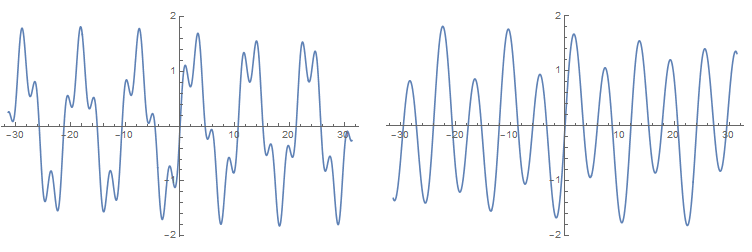
\includegraphics[width=\linewidth]{TwoSigmas.png}
%Plot[1/2 Cos[-1.3718298377306848` x] +   1.3228756555322954` Cos[-0.9348860049921902` x], {x, -10 Pi,   10 Pi}](*Sigma2=0.9*)
%Plot[1/2 Cos[-2.5082867902473156` x] +   1.3228756555322954` Cos[-0.4940354784643969` x], {x, -10 Pi,   10 Pi}](*Sigma2=0.2*)
  \caption{We show illustrative realisations of 1D functions. The left figure has a smaller $\gamma$ (larger $\sigma_2$) and more “short scale” power, allowing minima (maxima) to appear in significant numbers above (below) zero. When $\gamma$ is large (right figure) the spectrum is dominated by longer wavelength modes, and most minima are low-lying.}
  \label{examples1}
\end{figure}

We begin by making a qualitative exploration of the overall ``likelihood''. Firstly, we note that the integrand vanishes when any two ``adjacent'' $\lambda_i$ become equal, enforcing an ``eigenvalue repulsion'' in the Hessian matrices for the maxima and minima. This implies that a generic minima will be asymmetric, as their Hessians will have well separated eigenvalues.   

Secondly,  looking at Eq.~\ref{Q} we see that if $\gamma$ is close to unity,  the second term in $Q$ becomes very large, making the integrand a steeper function of the $x_i$ Conversely, if   $\gamma$ is small, $\nu$ can take larger values without dominating $Q$.  At larger values of $\gamma$ the power spectrum is effectively ``red'' and the random function is dominated by longer wavelength modes. By constrast, when $\gamma$ is small the spectrum is ``blue'' and dominated by shorter modes. In this case, it is more likely that extrema will be found at positive values of $\nu$. This behaviour is sketched in Fig~\ref{examples1} for illustrative one dimensional examples. 

Thirdly, as $N$ increases $Q$ will always grow, making it less likely to find minima and maxima on the ``wrong'' side of zero.

Finally, because we are interested in the regimes $\nu = 0 \ldots \infty$ and $\nu = -\infty \ldots \infty$, we can simplify the integral Eq. \ref{PminIntegral} by performing the $\nu$ integral analytically. The only dependence in the integrand on $\nu$ is in the first two terms of $Q$, which further remains the same for all $N$:

\begin{equation}
\begin{split}
\int^\infty_{-\infty} d\nu \int_{\lambda_1 \geq \lambda_2 \geq \lambda_3 \ldots \geq 0} G \times e^{-Q} dx_1  \cdots dx_N \\ 
= \int^\infty_{-\infty} d\nu e^{-\frac{\nu^2}{2}- \frac{(x- \gamma \nu)^2}{2(1-\gamma^2)}} \int_{\lambda_1 \geq \lambda_2 \geq \lambda_3 \ldots \geq 0} f(x_1, x_2 \ldots) dx_1  \cdots dx_N \\
= \int^\infty_{-\infty} d\nu e^{-\frac{x^2}{2}- \frac{(\nu - \gamma x)^2}{2(1-\gamma^2)}} \int_{\lambda_1 \geq \lambda_2 \geq \lambda_3 \ldots \geq 0} f(x_1, x_2 \ldots) dx_1  \cdots dx_N \\
= e^{-\frac{x^2}{2}} \sqrt{2\pi}\sqrt{1-\gamma^2}  \int_{\lambda_1 \geq \lambda_2 \geq \lambda_3 \ldots \geq 0} f(x_1, x_2 \ldots) dx_1  \cdots dx_N
\end{split}
\end{equation}

Similarly, 

\begin{equation}
\begin{split}
\int^\infty_0 d\nu \int_{\lambda_1 \geq \lambda_2 \geq \lambda_3 \ldots \geq 0} G \times e^{-Q} dx_1  \cdots dx_N \\ 
= e^{-\frac{x^2}{2}} \sqrt{\frac{\pi}{2}}\sqrt{1-\gamma^2} (1+\mathrm{Erf}(\frac{\gamma x}{\sqrt{2-2\gamma^2}})) \int_{\lambda_1 \geq \lambda_2 \geq \lambda_3 \ldots \geq 0} f(x_1, x_2 \ldots) dx_1  \cdots dx_N
\end{split}
\end{equation}

Although these analytic integrals are not always usable in what follows, when they are, they lighten the computational cost significantly.

\subsection{$N < 10$: Direct Evaluation  }

\begin{figure}
  \centering
  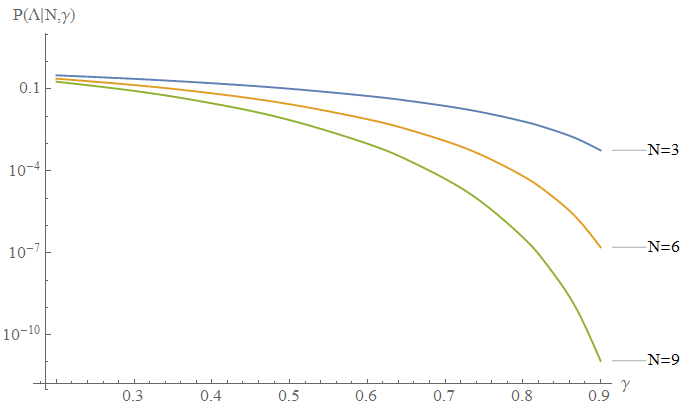
\includegraphics[width=\linewidth]{N369.png}
  \caption{The probability that a given minimum has $F > 0$ as a function of $\gamma$, for $N=3, 6, 9$. We can see that all the heuristics are obeyed: the probability decreases with $N$, and increases with $\sigma_2$.}
  \label{N6}
\end{figure}

\begin{figure}
  \centering
    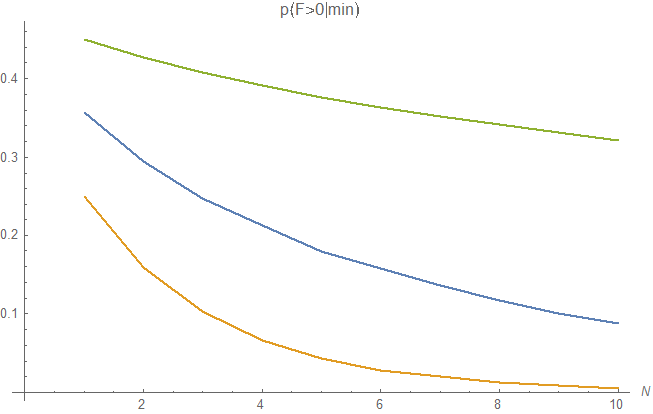
\includegraphics[width=\linewidth]{PVaryingWithN.png}
  \caption{A plot showing the value of $P(F>0|min)$ as a function of $N$ with $N\le10$, for $\gamma$ values $\frac{1}{5}, \frac{1}{3.5}$ and $\frac{1}{2}$ from top to bottom.}
  \label{gamma}
\end{figure}

For relatively small values of $N$ we can compute the integrals without any further approximations.   In Figs.~\ref{N6} and \ref{gamma}, we present $P(F>0|min)$ as a function of $N$ and $\gamma$. As expected, if the potential is highly oscillatory ($\sigma_2$ large, or $\gamma$ small), $P(F>0|min)$  tends towards 0.5 --  an equal likelihood of any given extremum being a maximum or a minimum. Conversely, if the potential is very smooth ($\sigma_2$ small; $\gamma$ very large), $P(F>0|min)$  tends towards 0. Moreover, for any given $\gamma$, $P(F>0|min)$ decreases with increasing $N$. 
 
%\begin{table}[h!] \label{Data}
%  \begin{center}
%    \caption{The probability that a given minimum has $\phi > 0$ as a function of $\sigma_2$. Values given for $N=4,5,6$ are exact; for larger values they are approximate (see the text; errors are on the order of the third nonzero digit after the decimal).}
%    \label{tab:table1}
%    \begin{tabular}{c|c|c} % <-- Alignments: center/center/center (l and r for left and right if needed)
%      $\textbf{N}$ & $\sigma_2$ & $p_{min}$\\
%      \hline
%      4 & 10 & 0.39141\\
%      5 & 10 & 0.37667\\
%      6 & 10 & 0.36320\\
%      7 & 10 & 0.35210\\
%      8 & 10 & 0.34227\\
%      9 & 10 & 0.33159\\
%      10 & 10 & 0.32151\\
%      \hline
%      4 & 3.5 & 0.21520\\
%      5 & 3.5 & 0.17886\\
%      6 & 3.5 & 0.15274\\
%      7 & 3.5 & 0.13599\\
%      8 & 3.5 & 0.11711\\
%      9 & 3.5 & 0.10093\\
%      10 & 3.5 & 0.08729\\
%      \end{tabular}
%      \quad
%      \begin{tabular}{c|c|c} 
%      $\textbf{N}$ & $\sigma_2$ & $p_{min}$\\
%      \hline
%      4 & 2 & 0.066638\\
%      5 & 2 & 0.043103\\
%      6 & 2 & 0.030844\\
%      7 & 2 & 0.02013\\
%      8 & 2 & 0.01307\\
%      9 & 2 & 0.00845\\
%      10 & 2 & 0.00544\\
%      \hline
%      4 & 1.25 & 0.001526\\
%      5 & 1.25 & 0.000327\\
%      6 & 1.25 & 6.53328 $\times 10^{-5}$\\
%      7 & 1.25 & 2.09673 $\times 10^{-5}$ \\
%      8 & 1.25 & 3.97235  $\times 10^{-6}$ \\
%      9 & 1.25 & 7.13489  $\times 10^{-7}$ \\
%      10 & 1.25 & 1.20253  $\times 10^{-7}$ \\
%     \end{tabular}
%  \end{center}
%\end{table}

%As can be seen, the probability that a given minimum has $\phi > 0$ decreases with increasing $N$. For a constant $\sigma_0$ and $\sigma_1$, the probability also decreases for increasing $\sigma_2$. Both of these general trends are to be expected: as $N$ increases, there are more conditions that must be simultaneously met for a point to be a minimum, hence the probability decreases. Also, since $\sigma_2$ is the average of the second derivative of the function, as $\sigma_2$ increases the function gets more and more turbulent. This means there are both more maxima and more minima, and the probability increases.

\subsection{$10 < N < \sim30$: Gaussian Approximations to the Integral}
For $N>10$, direct calculation becomes very resource-intensive. To proceed, we first select a value of the field $\nu$, then find the values of $x_1, x_2 \ldots$ that maximizes the integral in in Eq. \ref{DensityOfPeaks}. We then approximate the integral as a Gaussian integral about this maximum likelihood point:

\begin{align*}
\begin{split}
N &= A \int_{\lambda_1 \geq \lambda_2 \geq \lambda_3 \ldots \geq 0} F \times e^{-Q} dx dy dz \ldots \\
&=A\int_{\lambda_1 \geq \lambda_2 \geq \lambda_3 \ldots \geq 0} e^{\mathrm{log}F-Q} dx dy dz \ldots \\
&\approx \int_{-\infty}^{\infty} e^{-\frac{1}{2}xHx} d^nx = \sqrt{\frac{(2\pi)^n}{\mathrm{det} H}}
\end{split}
\end{align*}

\noindent where $H$ is the Hessian at the point being considered, and we no longer have an integral over $\nu$. This produces a list of points for each value of $\nu$. Fitting these points to a function and integrating that for the region with $\nu > 0$, we get an approximate result of the integral. \lfl{I feel like there's a more technical term for this, don't know what though.} This approximate value can then be compared against the exact value. The Gaussian approximation turns out to be very good (see Fig. \ref{Comparison}). The Gaussian integral can be more efficiently computed than Eq. \ref{DensityOfPeaks}, which lets us evaluate it up to $N\approx30$.

The plot of the logarithms of these results against the number of dimensions is surprisingly straight (Fig. \ref{PVaryingWithNGaussian}). Although it is not conclusive,\footnote{Per Figure 4 of \cite{Yamada2018}, it is possible the behavior of the function changes at $N >100$.} it is suggestive.

\subsection{$\sim 30 < N < \sim100$: Approximations using the $\nu=0$ point}

The Gaussian approximation described in the previous subsection requires the integral to be computed for several different values of $\nu$. If we use only the result at the $\nu=0$ point, we get a result that is much larger than the exact results, but it remains at a nearly-constant ratio to it (see Fig. sigma2=2v=0). Using this, we confirm that the straight line behavior holds up to $N = 100$.

\begin{figure} 
  \centering
  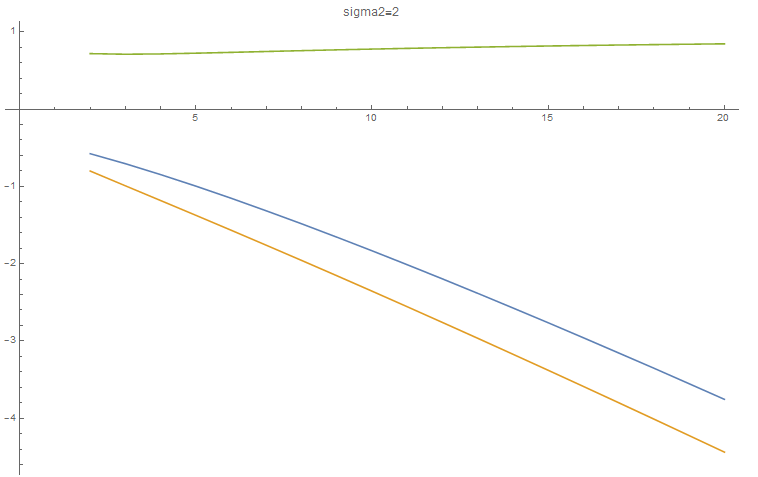
\includegraphics[width=\linewidth]{sigma2=2v=0.png}
  \caption{A comparison of the Gaussian approximation evaluated at the $\nu=0$ point to the full integral. The blue line corresponds to the $\nu=0$ results, while the orange line corresponds to the Gaussian results (Section 3.3). Horizontal axis is $N$ while the vertical axis is the $Log_{10}$ of the probability. The $\nu=0$ results are always larger than the actual results, but the ratio of their logarithms is approximately constant.}
  \label{sigma2=2v=0}
\end{figure}

Based on these calculations, we conclude that the value of $\sigma_2$ for which $P(F>0|min)$ drops to $\sim 10^{-500}$ at $N = 100$ is about $1.08$. In other words, there will be plenty of minima in the landscape that could correspond to our universe if the landscape has $\sigma_2 \gtrapprox 1.08$ (with $\sigma_0$ and $\sigma_1$ normalized to 1).

\begin{figure} 
  \centering
  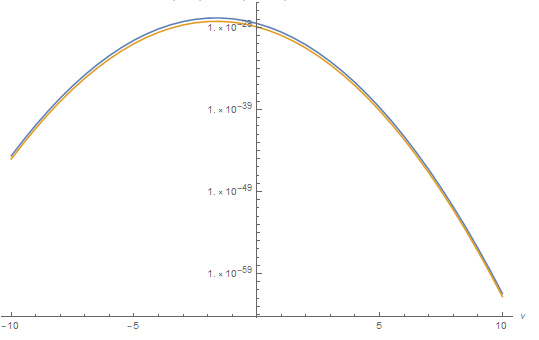
\includegraphics[width=\linewidth]{Comparison.png}
  \caption{A comparison of $P(F)$ with the Gaussian approximation, at specified values of $\nu$ ($N=8$). Blue line corresponds to the Gaussian results, while the orange line corresponds to the exact integral. Horizontal axis is $\nu$ while the vertical axis is (unormalized) likelihood. As expected, because the Gaussian integral integrates to infinity while the exact integral does not, it yields a larger likelihood.}
  \label{Comparison}
\end{figure}

\begin{figure} 
  \centering
  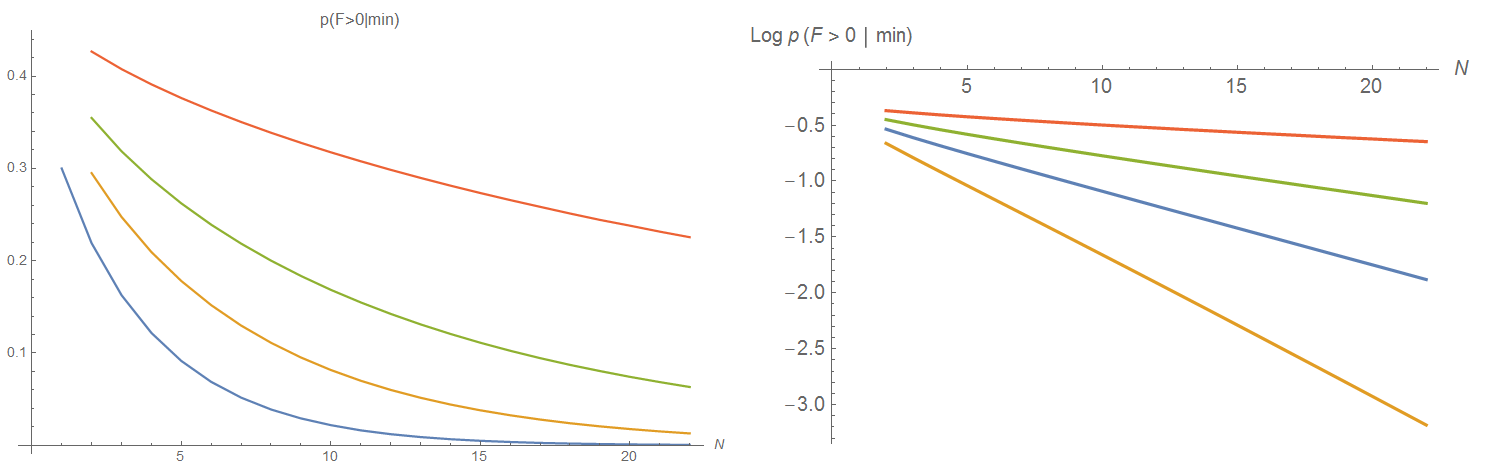
\includegraphics[width=\linewidth]{PVaryingWithNGaussian.png}
  \caption{(Left) The probability of a minimum above $\nu=0$, calculated using the Gaussian approximation. The lines correspond to $\gamma = \frac{1}{10}, \frac{1}{5}, \frac{1}{3.5}, \frac{1}{2.5}$ respectively from top to bottom. Compare Fig. \ref{gamma}. (Right) The same data, plotted using a different y-axis ($Log$ here is to base 10). All four lines yield a logarithm well above $-500$ at $N=100$. The cutoff at which $p(F>0|min) \sim 10^{-500}$, with $\sigma_0$ and $\sigma_1$ normalized to 1,  is $\sigma_2 \approx 1.08$.}
  \label{PVaryingWithNGaussian}
\end{figure}

%We have tried two ways to do this.

%The first way is to extrapolate from the data in Table \ref{Data}. In Fig. \ref{Log-Linear}, we present a log-linear plot of the probability against the dimension for the three values of $\sigma_2$. The resulting lines are surprisingly straight. There is a noticeable kink in both the $\sigma_2 = 3.5$ and $\sigma_2=2$ case between $N=6$ and $N=7$. This is a numerical effect -- it is where the exact results end and the numerical ones begin. If the trend is robust, then for the case of $\sigma_2=2$, the probability at $N=100$ is of the order of $p \sim 10^{-42}$. Since there are $\sim 10^{500}$ stationary points in the landscape,\cite{Douglas} this probability, while small, still leads to there being $\sim 10^{458}$ minima that might correspond to our universe.

%We checked this by running the numerical integration for $N=6$ as well. Replacing the exact result with the numerical one, the kink moves to the left. The kink indicates that the numerical results are consistently overestimating the true probability, but that is not surprising because the numerical results rely on the trapezoidal rule. The trapezoidal rule overestimates the result when the integral is concave up, and underestimates it when it is concave down. The final probability is the area under the curve for $\phi > 0$ divided by the area under the curve for all $\phi$. From Fig. \ref{Likelihood}, for $\phi > 0$ the curve is concave up, so the trapezoidal rule overestimates the numerator, and accordingly the probability as well. This trend holds for higher $N$ as well, since for higher $N$ the plot moves to more negative values.

%\begin{figure}
%  \centering
%  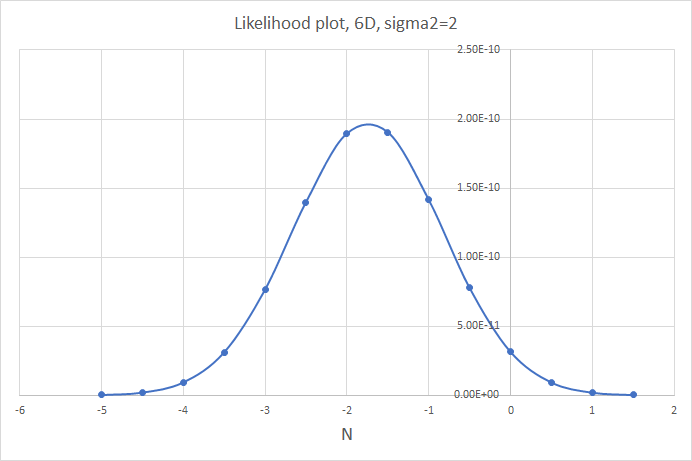
\includegraphics[width=\linewidth]{LikelihoodPlot.png}
%  \caption{A plot of the likelihood for $\sigma_2=2, N=6$. The final probability desired is the area under the curve for $\phi > 0$ divided by the area unde the curve for all $\phi$. For the region $\phi > 0$, the curve is concave upwards, so the trapezoidal rule overestimates its value. Accordingly, the numerator and probability are also overestimated.}
%  \label{Likelihood}
%\end{figure}

%The other way is to with ratios of the peak likelihood. The idea is to take the logarithm of the integrand in Eq. \ref{DensityOfPeaks}, which results in a function $G(x, y, z, \ldots)$, and then find the values of $x, y, z \ldots$ which maximizes this integrand. This corresponds to the single most likely point. Having done this, we can compute the ratio of this maximum vs. the point $\phi = 0$, which is a number much more easily calculated. The result in 4D is show in Fig. \ref{LogRatioNoFit}. It's obvious that the blue line is not a good fit of the orange line, but it takes the same shape. Since string theory predicts a truly gargantuan number of stationary points -- on the order of $10^{500}$ -- being off by even $\sim100$ orders of magnitude is not necessarily fatal.

%\begin{figure}
%  \centering
%  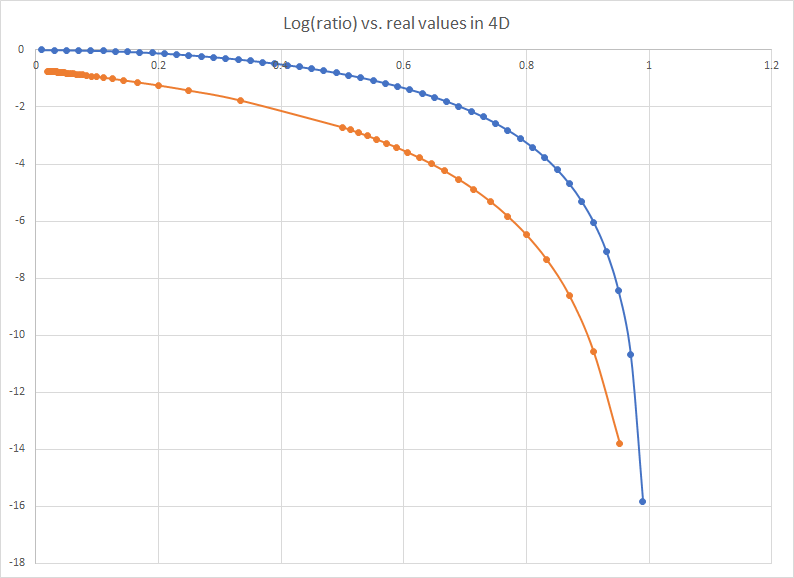
\includegraphics[width=\linewidth]{LogRatioNoFit.png}
%  \caption{Plot of the logarithm of the ratio of likelihood for the overall peak to the point $\phi = 0$ as a function of $\gamma$, as well as the analytic results, in 4 dimensions. The blue line is the logarithm of the ratio of likelihood, the orange line is the analytic results.}
%  \label{LogRatioNoFit}
%\end{figure}

\section{Implications for Multiverse Cosmology}

\re{I would move from looking at the abstract problem in the previous section to the specific implications for cosmology in this section; and how $P(\Lambda)$ depends on $\sigma_2$}

\lfl{Dunno what to put here anymore}

\section{Conclusion}
We have presented results for the statistics of stationary points at a given function value as a function of $N$ and $\sigma_2$. The numbers confirm the intuitive expectation that the probability of a given extremum with $F > 0$ being a minimum decreases as $N$ increases or as $\sigma_2$ decreases. We are able to calculate precise values for the probability up to $N=10$. Above this dimension, evaluating Eq. \ref{DensityOfPeaks} is computationally prohibitive, but we find that Eq. \ref{DensityOfPeaks} is well-approximated by a Gaussian integral. Using this approximation, we are able to estimate the probability up to $N \approx 30$. For $N>30$, we use only the $\nu=0$ point, which although much smaller than the actual results, remains in roughly constant ratio with it. The final probability as a function of $N$ is well-approximated by a straight line when plotted on a logarithmic scale for various values of $\sigma_2$ (Fig. \ref{PVaryingWithNGaussian}). If this trend holds to larger values of $N$, we estimate that the value of $\sigma_2$ for which $P(F>0|min)$ drops to $\sim 10^{-500}$ is approximately $1.08$.

The results of this paper establish the number of vacua that could correspond to our universe in string theory, but does not treat the distribution of eigenvalues -- and accordingly the duration of slow-roll inflation -- that could arise from these vacua. An analysis of this will be the focus of future work.

\section{Appendix}
\subsection{Density of peaks for $N=4$} 
For $N=4$, the full result of the integral Eq. \ref{DensityOfPeaks} is:

\begin{equation}
\begin{split}
N = \frac{1}{214990848} \mathrm{Exp}\frac{9x^2\sigma_1^4 + 2\nu x \sigma_0 \sigma_1^2 \sigma_2 - (v^2+10x^2)\sigma_0^2\sigma_2^2}{-2\sigma_1^4+2\sigma_0^2\sigma_2^2}\\\bigg{(}80x - 1610e^{3x^2}+128x^3+418e^{3x^2}x^3+4e^{4x^2}\sqrt{\pi}(3+48x^2+64x^4)\mathrm{Erf}\bigg{[}\sqrt{\frac{3}{2}}x\bigg{]}\\
-486e^{\frac{9x^2}{2}}\sqrt{6\pi}x^2\mathrm{Erf}\bigg{[}\sqrt{\frac{3}{2}}x\bigg{]}+81e^{\frac{9x^2}{2}}\sqrt{6\pi}x^4\mathrm{Erf}\bigg{[}\sqrt{\frac{3}{2}}x\bigg{]}\bigg{)}
\end{split}
\end{equation}

The higher-dimensional results take the same form: an overall exponential multiplied by a product of polynomials and error functions; however they are massive (for example, in 5D there are some eight hundred terms).

\subsection{$p(F|s.p.)$ for $N=2$}
The full expression for $p(F|s.p.)$ in 2D is:

\begin{equation}
\begin{split}
p(F|s.p.)=\frac{\sqrt{\pi}}{4\sqrt{4\gamma^2-6}}\bigg{[}\mathrm{Exp}\frac{F^2}{2(\gamma^2-1)}\bigg{(}2\mathrm{Exp}\bigg{(}\frac{F^2\gamma^2}{e^6-10\gamma^2+4\gamma^4}\bigg{)}\sqrt{\gamma^2-1}\\
-\mathrm{Exp}\bigg{(}\frac{F^2\gamma^2}{2-2\gamma^2}\bigg{)}(F^2-1)(\gamma^2-1)\gamma^2\sqrt{\frac{2\gamma^2-3}{1-\gamma^2}}\bigg{)}\bigg{]}
\end{split}
\end{equation}

\noindent where $\gamma = \sigma_1^2/\sigma_0\sigma_2$. This result can be derived using a similar method as to derive Eq. \ref{DensityOfPeaks}, but by relaxing the requirement that the smallest eigenvalue is greater than zero.

\begin{thebibliography}{99}
\bibitem{Planck2018} Planck Collaboration 2018 results. Submitted to \emph{Astronomy \& Astrophysics}.
\bibitem{DES} Dark Energy Survey year 1 results. arXiv:1802.05257
\bibitem{Linde1986} A. D. Linde, Phys. Lett. B 175, 4, 395--400, 1986
\bibitem{Adshead2007} P. Adshead, R. Easther, and E. A. Lim, Phys. Rev. D 79, 063504, 2009
\bibitem{Guth2001} A. Guth, arXiv: astro-ph/0101507
\bibitem{Susskind2003} L. Susskind, arXiv:hep-th/0302219
\bibitem{Bousso2000} R. Bousso and J. Polchinski, Journal of High Energy Physics, 06, 006, 2000
\bibitem{Agrawal2018} P. Agrawal, G. Obied, P. J. Steinhardt, C. Vafa, Physics Letters B, 784, 271--276, 2018
\bibitem{GRF1} A. Masoumi, A. Vilenkin and M. Yamada, Journal of Cosmology and Astroparticle Physics, 05:053, 2017
\bibitem{GRF2} A. Masoumi, A. Vilenkin and M. Yamada, Journal of Cosmology and Astroparticle Physics, 12:035, 2017
\bibitem{GRF3} T. Bjorkmo and M.C.D. Marsh, Journal of Cosmology and Astroparticle Physics, 02:037, 2018
\bibitem{Aazami2006} A. Aazami and R. Easther, Journal of Cosmology and Astroparticle Physics (0603:013), 2006
\bibitem{Bray2007} A. J. Bray and D. S. Dean, Physical Review Letters, 98, 150201, 2007
\bibitem{Easther2006} R. Easther and L. McAllister, Journal of Cosmology and Astroparticle Physics 05:018, 2006
\bibitem{Frazer2011} J. Frazer and A. R. Liddle, Journal of Cosmology and Astroparticle Physics 02:026, 2011
\bibitem{Henry2009} S.-H. Henry Tye, J. J. Xu and Y. Zhang, Journal of Cosmology and Astroparticle Physics 04:018, 2009
\bibitem{Marsh2013} M.C.D. Marsh, L. McAllister, E. Pajer and T. Wrase, Journal of Cosmology and Astroparticle Physics 11:040, 2013
\bibitem{Agarwal2011} N. Agarwal, R. Bean, L. McAllister and G. Xu, Journal of Cosmology and Astroparticle Physics 09:002, 2011
\bibitem{Yang2012} I.S. Yang, Physical Review D, 86, 103537, 2012
\bibitem{Masoumi2016} A. Masoumi and A. Vilenkin, Journal of Cosmology and Astroparticle Physics 03:054, 2016
\bibitem{Yamada2018} M. Yamada and A. Vilenkin, Journal of High Energy Physics 2018: 29, 2018
\bibitem{Fyodorov2004} Y. V. Fyodorov, Physical Revew Letters, 92, 240601, 2004
\bibitem{Douglas2004} M. R. Douglas, B. Shiffman and S. Zelditch, Communications in Mathematical Physics, 252, 325, 2004
\bibitem{Douglas2006} M. R. Douglas, B. Shiffman and S. Zelditch, Communications in Mathematical Physics, 265, 617, 2006 
\bibitem{Fyodorov2007} Y. V. Fyodorov and I. Williams, Journal of Statistical Physics, 129, 5, 2007
\bibitem{Fyodorov2012} Y. V. Fyodorov and C. Nadal, Physical Review Letters, 109, 167203, 2012
\bibitem{Fyodorov2018} Y. V. Fyodorov, P. L. Doussal, A. Rosso, C. Texier, Annals of Physics, 397, 2018
\bibitem{Ros2019}  V. Ros, G. B. Arous, G. Biroli and C. Cammarota, Physical Review X 9, 011003
\bibitem{Dean2008} D. S. Dean and S. N. Majumdar, Physical Review E., 77, 041108, 2008
\bibitem{Majumdar2009} S. N. Majumdar, C. Nadal, A. Scardicchio, and P. Vivo., Physical Review Letters, 103, 220603, 2009
\bibitem{Bachlechner2014} T.C. Bachlechner, Journal of High Energy Physics, 2014: 54, 2014
\bibitem{Battefeld2012} D. Battefeld, T. Battefeld, S. Schulz, Journal of Cosmology and Astroparticle Physics, 06:034, 2012
\bibitem{Fyodorov2013} Y. V. Fyodorov, Markov Processes Relat. Fields, 21, 483--51, 2015
\bibitem{Masoumi2017} A. Masoumi, M. Yamada and A. Vilenkin, Journal of Cosmology and Astroparticle Physics, 07:003, 2017
\bibitem{Easther2016} R. Easther, A. Guth and A. Masoumi, arXiv:1612.05224 (2016)
\bibitem{Kac1943} M. Kac, \emph{Bull. Amer. Math. Soc.}, 43, 314–320, 1943
\bibitem{Rice1945}  S. O. Rice, \emph{Bell System Tech. J.}, 24, 46--156, 1945
\bibitem{BBKS} J. M. Bardeen, J. R. Bond, N. Kaiser, and A. S. Szalay, Astrophysical Journal, Astrophysical Journal, vol. 304, page 15-61 (1986)
\bibitem{Goldstein} See e.g. H. Goldstein, C. P. Poole, and J. L. Safko, \emph{Classical Mechanics 3rd ed.}, Pearson (2001)
\bibitem{VEGAS} G. P. Lepage, Journal of Computational Physics 27, 192, 1978.
\bibitem{GSL} B. Gough, \emph{GNU Scientific Library Reference Manual - Third Edition, 3rd ed.} (Network Theory Ltd., 2009).
\bibitem{Douglas2003} M. R. Douglas, Journal of High Energy Physics, 05:046, 2003
\end{thebibliography}

\end{document}